\documentclass[a4paper, 12pt]{article}
\usepackage[left=1.5cm, right=1.5cm, top=1.5cm, bottom=2.5cm]{geometry}
\usepackage[utf8]{inputenc}
\usepackage[russian]{babel}
\usepackage{verbatim}
\usepackage{graphicx}
\usepackage{listingsutf8}
\usepackage{color}
\usepackage{ulem}
\usepackage{amsmath}
\usepackage{array}
\usepackage{amssymb, latexsym, amsmath, textcomp}
\usepackage{indentfirst}
\usepackage{cmap}
\usepackage{graphics}
\usepackage{listings}
\usepackage{enumerate}

\lstset{
basicstyle=\footnotesize,
breaklines=true,
numbers=left,
extendedchars=\true,
numbersep=7pt,
caption=\lstname,
frame=single,
inputencoding=utf8,
showstringspaces=\false
}

\newenvironment{enumerate*}%
  {\begin{enumerate}%
    \setlength{\itemsep}{1pt}%
    \setlength{\parskip}{1pt}}%
  {\end{enumerate}}
\newenvironment{itemize*}%
  {\begin{itemize}%
    \setlength{\itemsep}{1pt}%
    \setlength{\parskip}{1pt}}%
  {\end{itemize}}

%------------------------------------------------------------------------------------------------------------------------------
%------------------------------------------------------------------------------------------------------------------------------
\begin{document}

\begin{titlepage}
\begin{center}
{Санкт-Петербургский национальный исследовательский университет информационных технологий, механики и оптики}

Кафедра вычислительной техники
\end{center}
\vspace{50mm}
\begin{center}
\begin{tabular}{c}
\Huge{\textbf{Отчёт}}\\
\Large{\textbf{по лабораторной работе №2}}\\
\Large{\textbf{дисциплины <<Программирование интернет-приложений>>}}\\
\Large{\textbf{Вариант №355}}\\[2mm]
\end{tabular}
\end{center}
\vspace{85mm}
\begin{flushright}
\begin{tabular}{l}
Выполнили:\\
студенты гр. P3211\\
Ефремов Р.В.,\\
Синицкий Д.П.\\
Преподаватели:\\
Цопа Е.А.\\
Письмак А.Е.\\
\\
\end{tabular}
\end{flushright}
\vspace{15mm}
\begin{center}
Санкт-Петербург - 2017 г.
\end{center}
\end{titlepage}
\newpage

\section{Текст задания}

Разработать веб-приложение на базе сервлетов и JSP, определяющее попадание точки на координатной плоскости в заданную область.

Приложение должно быть реализовано в соответствии с шаблоном MVC и состоять из следующих элементов:


\begin{itemize*}
\item ControllerServlet, определяющий тип запроса, и, в зависимости от того, содержит ли запрос информацию о координатах точки и радиусе, делегирующий его обработку одному из перечисленных ниже компонентов. Все запросы внутри приложения должны передаваться этому сервлету (по методу GET или POST в зависимости от варианта задания), остальные сервлеты с веб-страниц напрямую вызываться не должны.
\item AreaCheckServlet, осуществляющий проверку попадания точки в область на координатной плоскости и формирующий HTML-страницу с результатами проверки. Должен обрабатывать все запросы, содержащие сведения о координатах точки и радиусе области.
\item Страница JSP, формирующая HTML-страницу с веб-формой. Должна обрабатывать все запросы, не содержащие сведений о координатах точки и радиусе области.

\end{itemize*}

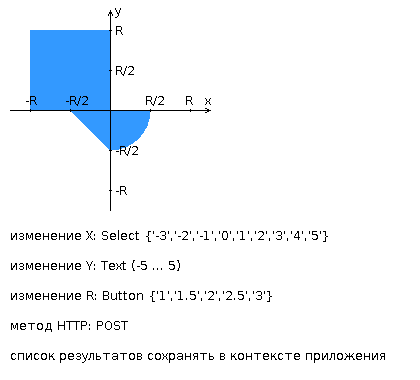
\includegraphics[scale=0.7]{img/areas.png}

\paragraph{Разработанная страница JSP должна содержать:}
\begin{enumerate*}
\item ''Шапку'', содержащую ФИО студента, номер группы и номер варианта.
\item Форму, отправляющую данные на сервер.
\item Набор полей для задания координат точки и радиуса области в соответствии с вариантом задания.
\item Сценарий на языке JavaScript, осуществляющий валидацию значений, вводимых пользователем в поля формы.
\item Интерактивный элемент, содержащий изображение области на координатной плоскости (в соответствии с вариантом задания) и реализующий следующую функциональность:
\begin{itemize*}
\item Если радиус области установлен, клик курсором мыши по изображению должен обрабатываться JavaScript-функцией, определяющей координаты точки, по которой кликнул пользователь и отправляющей полученные координаты на сервер для проверки факта попадания.
\item В противном случае, после клика по картинке должно выводиться сообщение о невозможности определения координат точки.
\item После проверки факта попадания точки в область изображение должно быть обновлено с учётом результатов этой проверки (т.е., на нём должна появиться новая точка).
\end{itemize*}
\item Таблицу с результатами предыдущих проверок. Список результатов должен браться из контекста приложения, HTTP-сессии или Bean-компонента в зависимости от варианта.
\end{enumerate*}

\paragraph{Страница, возвращаемая AreaCheckServlet, должна содержать:}

\begin{enumerate*}
	\item Таблицу, содержащую полученные параметры.
	\item Результат вычислений - факт попадания или непопадания точки в область.
	\item Ссылку на страницу с веб-формой для формирования нового запроса.
\end{enumerate*}

Разработанное веб-приложение необходимо развернуть на сервере GlassFish.


\section{Код}

\lstinputlisting[language=HTML, caption=index.jsp{../web/content/index.jsp}
\lstinputlisting[language=Java, caption=AreaCheckServlet.java]{../src/AreaCheckServlet.java}
\lstinputlisting[language=Java, caption=ControllerServlet.java]{../src/ControllerServlet.java}
\lstinputlisting[language=Java, caption=Point.java]{../src/Point.java}
\lstinputlisting[caption=web.xml]{../web/WEB-INF/web.xml}

\section{Выводы по работе}
% В ходе подготовки к выполнению данной лабораторной работы были изучены основы <...>

% С использованием полученных знаний в соответствии с заданием была реализована <...>

\end{document}
